\lstset{
  basicstyle=\ttfamily,
  columns=fullflexible,
  frame=single,
  breaklines=true,
  showlines=true,
  postbreak=\mbox{\textcolor{red}{$\hookrightarrow$}\space},
}

\chapter{Implementasi dan Pengujian}
\label{chap:implementasiDanPengujian}

Bab ini membahas proses implementasi dan proses pengujian fitur Kolektor Pengumuman Informatika.
\section{Implementasi}
Bagian ini membahas implementasi dari perancangan yang telah dilakukan di Bab 3.
\subsection{Lingkungan Pengembangan}
Berikut spesifikasi perangkat keras dan perangkat lunak yang dipakai untuk pengembangan pada skripsi ini :

\textbf{Spesifikasi Perangkat keras}
\begin{itemize}
\item Processor Intel® Celeron(R) CPU 1007U @ 1.50GHz x 2 
\item Graphics Intel® Ivybridge Mobile
\item RAM 8 GB
\item Harddisk 500GB SATA
\item Wireless keyboard and mouse combo Logitech MK215
\end{itemize}

\textbf{Spesifikasi Perangkat lunak}
\begin{itemize}
\item Sistem Operasi Ubuntu 18.04.1 LTS 64-bit
\item Visual Studio Code version 1.31.0
\item apache2 -v
\item PHP 7.2.10 (cli)
\item Composer version 1.7.2
\item pgAdmin4 version 2.1 (Application Mode : Desktop)
\item psql (PostgreSQL) 10.6
\item heroku/7.21.0 linux-x64 node-v11.9.0
\end{itemize}

\subsection{Implementasi Basis Data}
Pada pembangunan fitur Kolektor Pengumuman Informatika, ada dua tabel yang ditambahkan. Kedua tabel itu adalah tabel Pengumuman dan tabel PengumumanLineFollowers. Pembuatan tabel menggunakan dua file migration terpisah : file 20181011103200\_Pengumuman\_Initial.php dan 20190210224400\_PengumumanLineFollowers\_initial.php.

\subsection{Implementasi Kelas}
Pada pembangunan fitur Kolektor Pengumuman Informatika, dibuat kelas-kelas berikut : 
\begin{itemize}
\item Kelas model Pengumuman\_model

Pengumuman\_model merupakan kelas yang berisi algoritma yang dibutuhkan oleh fitur Kolektor Pengumuman Informatika.

\item Kelas model Pengumuman\_Line\_model

Pengumuman\_model merupakan kelas yang dikhususkan untuk algoritma untuk menghubungkan BlueTape dengan LINE API.

\item Kelas controller Cron

Cron merupakan kelas yang berfungsi untuk menjalankan perintah-perintah yang harus dijalankan pada jadwal tertentu. Pada skripsi ini perintah yang dijadwalkan adalah memeriksa email. Pada tahap perancangan, perintah untuk memeriksa email dijadwalkan tiap lima belas menit. Namun, karena keterbatasan dana, perintah ini dijadwalkan tiap hari pada jam 12 tepat siang.

\item Kelas controller Pengumuman

Pengumuman merupakan kelas yang berfungsi untuk mengatur hubungan antara Pengumuman\_model dan view yang ada di package Pengumuman.

\item Kelas controller PengumumanLine

Pengumuman\_Line merupakan kelas yang berfungsi untuk menerima webhook dari LineAPI.

\end{itemize}

Untuk mendukung kinerja kelas-kelas tersebut, dibuat juga file :
\begin{itemize}
\item File view main.php.

File ini digunakan untuk mengatur tampilan halaman utama Pengumuman.

\item File view read.php.

File ini digunakan untuk mengatur tampilan halaman saat detail pengumuman ditampilkan.

\item File config pengumuman.php.

File ini digunakan untuk menyimpan daftar pengirim pengumuman yang terverifikasi.

\item File migration 20181011103200\_Pengumuman\_Initial.php 

File ini digunakan untuk membuat tabel Pengumuman.

\item File migration 20190210224400\_PengumumanLineFollowers\_initial.php.

File ini digunakan untuk membuat tabel PengumumanLineFollowers.
\end{itemize}

Selain itu, ada beberapa file yang harus diubah :
\begin{itemize}
\item file config database.php

Pada file ini informasi database disesuaikan dengan informasi database yang dipakai di skripsi ini.

\item file config modules.php

Pada file ini ditambahkan modules Pengumuman pada config 'modules'.

\item file config routes.php

Pada file ini ditambahkan routing berikut :
\begin{lstlisting}
$route['pengumuman/page-(:num)'] = '/pengumuman/page/$1';
\end{lstlisting}
\end{itemize}

\section{Pengujian}
\subsection{Lingkungan Pengujian}
Berikut spesifikasi yang dipakai untuk pengujian pada skripsi ini :
\begin{itemize}
\item Heroku dengan spesifikasi :

\begin{itemize}
\item Region : United States
\item Stack : heroku-18
\item Framework : PHP
\item Maximum Slug Size : 500 MiB
\item Heroku Git URL : https://git.heroku.com/shadowtape.git
\item Buildpack : heroku/php
\item Domain : https://shadowtape.herokuapp.com/
\item Dyno Type : Free Dynos
\item Add-ons Heroku Postgres dan Heroku Scheduler
\end{itemize}

\item Bot LINE dengan plan Developer
\end{itemize}

\subsection{Pengujian Fungsional}
Pengujian fungsional dilakukan dengan metode black box testing. Berikut adalah hasil pengujiannya :
\begin{itemize}
  \item Pengujian Filter Email Pengumuman

    Pengujian ini bertujuan untuk menguji apakah filter email pengumuman berfungsi dengan baik. Email yang dikirim di pengujian ini memiliki subjek. Hasil pengujian dapat dilihat di Tabel \ref{table:pengujian-fungsional-filter-email}.

    \begin{center}
      \begin{table}[H]
        \caption{Pengujian Filter Email Pengumuman}
        \label{table:pengujian-fungsional-filter-email}
        \begin{tabular}{|p{5cm}|p{5cm}|p{5cm}|}
        \hline
        \centering Aksi	& 	\centering Reaksi yang diharapkan &  \multicolumn{1}{c|}{Reaksi Perangkat Lunak} \\
        \hline
        Mengirimkan email dengan email yang terdaftar lalu menjalankan Cron. & Email masuk ke database dan pengumuman ditampilkan di menu pengumuman. & Reaksi sesuai dengan yang diharapkan. Email masuk ke database dan pengumuman dapat dilihat di menu pengumuman. \\
        \hline
        Mengirimkan email dengan email yang tidak terdaftar lalu menjalankan Cron. & Email tidak masuk ke database. & Reaksi sesuai dengan yang diharapkan. Email tidak masuk ke database. \\
        \hline
        \end{tabular}
    \end{table}
    \end{center}

  \item Pengujian Mengirim Email dengan Isi Email yang Variatif

    Pengujian ini bertujuan untuk menguji apakah isi email yang ditampilkan sesuai dengan yang diharapkan. Pengujian ini dilakukan dengan mengirimkan beberapa email dengan isi yang berbeda melalui email yang terdaftar di BlueTape. Hasil pengujian dapat dilihat di Tabel ~\ref{table:pengujian-fungsional-isi-variatif}.

      \begin{longtable}{|p{5cm}|p{5cm}|p{5cm}|}
        \caption{Pengujian Mengirim Email dengan Isi Email yang Variatif}
        \label{table:pengujian-fungsional-isi-variatif}\\
        \hline
        \centering Aksi	& 	\centering Reaksi yang diharapkan &  \multicolumn{1}{c|}{Reaksi Perangkat Lunak} \\
        \hline
        Mengirimkan email tanpa subjek lalu menjalankan Cron. & Email tidak masuk ke database. & Reaksi sesuai dengan yang diharapkan. Email tidak masuk ke database. \\
        \hline
        Mengirimkan email tanpa isi lalu menjalankan Cron. & Email masuk ke database dan pengumuman ditampilkan di menu pengumuman. & Reaksi sesuai dengan yang diharapkan. Email masuk ke database dan pengumuman dapat dilihat di menu pengumuman. \\
        \hline
        Mengirimkan email dengan subjek dan isi lalu menjalankan Cron. & Email masuk ke database dan pengumuman ditampilkan di menu pengumuman. & Reaksi sesuai dengan yang diharapkan. Email masuk ke database dan pengumuman dapat dilihat di menu pengumuman. \\
        \hline
        Mengirimkan email balasan lalu menjalankan Cron. & Email masuk ke database dan pengumuman ditampilkan di menu pengumuman. & Reaksi sesuai dengan yang diharapkan. Email masuk ke database dan pengumuman dapat dilihat di menu pengumuman. \\
        \hline
        Mengirimkan email terusan lalu menjalankan Cron. & Email masuk ke database dan pengumuman ditampilkan di menu pengumuman. & Reaksi sesuai dengan yang diharapkan. Email masuk ke database dan pengumuman dapat dilihat di menu pengumuman. \\
        \hline
        Mengirimkan email dengan lampiran lalu menjalankan Cron. & Email masuk ke database dan pengumuman ditampilkan di menu pengumuman. Di bawah isi pengumuman, ada keterangan "*) Pengumuman ini memiliki lampiran, silahkan memeriksa langsung email student Anda untuk mengunduhnya.". & Reaksi sesuai dengan yang diharapkan. Email masuk ke database dan pengumuman dapat dilihat di menu pengumuman. Di bawah isi pengumuman, keterangan "*) Pengumuman ini memiliki lampiran, silahkan memeriksa langsung email student Anda untuk mengunduhnya." berhasil ditampilkan. \\
        \hline
        Mengirimkan email yang terdapat sisipan lampiran berupa gambar di isi email lalu menjalankan Cron. & Email masuk ke database dan pengumuman ditampilkan di menu pengumuman. Di bawah isi pengumuman, ada keterangan "*) Pengumuman ini memiliki lampiran, silahkan memeriksa langsung email student Anda untuk mengunduhnya.". Isi pesan harus masih lengkap walaupun gambar tidak akan berhasil ditampilkan (karena file gambar tidak bisa disimpan di server). & Reaksi sesuai dengan yang diharapkan. Email masuk ke database dan pengumuman dapat dilihat di menu pengumuman. Di bawah isi pengumuman, keterangan "*) Pengumuman ini memiliki lampiran, silahkan memeriksa langsung email student Anda untuk mengunduhnya." berhasil ditampilkan. Isi pesan lengkap. Sesuai ekspektasi, gambar tidak bisa ditampilkan. Namun, ada keterangan alt yang berisi nama file.\\
        \hline
        Mengirimkan email yang isinya memakai berbagai jenis pemformatan yang bisa dilakukan di gmail, emoji yang disediakan gmail, dan sisipan url. Setelah itu menjalankan Cron. & Email masuk ke database dan pengumuman ditampilkan di menu pengumuman. Isi email lengkap. Pemformatan tetap sama. Emoji tidak diharapkan bisa ditampilkan. Sisipan url dapat ditampilkan dan url dapat dikunjungi. & Reaksi sesuai dengan yang diharapkan. Email masuk ke database dan pengumuman dapat dilihat di menu pengumuman. Isi email lengkap. Pemformatan tetap sama. Emoji dapat ditampilkan. Beberapa emoji berubah bentuk namun tetap memiliki bentuk yang sama. Beberapa emoji persis sama dengan yang ada di isi email yang asli. Sisipan url dapat ditampilkan dan url dapat dikunjungi. \\
        \hline
    \end{longtable}

    \item Pengujian Notifikasi LINE

    Pengujian ini bertujuan untuk menguji apakah notifikasi LINE dapat terkirim ke bot LINE. Tabel \ref{table:pengujian-fungsional-notifikasi-line}.

    \begin{center}
      \begin{table}[H]
        \caption{Pengujian Notifikasi LINE}
        \label{table:pengujian-fungsional-notifikasi-line}
        \begin{tabular}{|p{5cm}|p{5cm}|p{5cm}|}
        \hline
        \centering Aksi	& 	\centering Reaksi yang diharapkan &  \multicolumn{1}{c|}{Reaksi Perangkat Lunak} \\
        \hline
        Follow akun bot. & User Id LINE tercatat di database. & Reaksi sesuai dengan yang diharapkan. User Id LINE berhasil tercatat di database.\\
        \hline 
        Mengirimkan email dengan email yang terdaftar lalu menjalankan Cron. Email harus memiliki subjek. & Setelah Cron sukses dijalankan, notifikasi LINE dari akun bot muncul. & Reaksi sesuai dengan yang diharapkan. Notifikasi LINE dari akun bot muncul. \\
        \hline
        Membuka pesan LINE yang masuk. Setelah itu membuka url yang tercantum di pesan. & URL dapat dibuka. Apabila belum login ke BlueTape, pengguna akan diarahkan ke menu login. Setelah login, pengguna diarahkan kembali ke URL tersebut. & Reaksi sesuai dengan yang diharapkan. URL dapat dibuka. Apabila belum login ke BlueTape, pengguna akan diarahkan ke menu login. Setelah login, pengguna diarahkan kembali ke URL tersebut.  \\
        \hline
        \end{tabular}
    \end{table}
    \end{center}
\end{itemize}


\subsection{Pengujian Eksperimental}
Pengujian eksperimental untuk aplikasi ini dilakukan pada mata kuliah AIF182100 (Analisis dan Desain Perangkat Lunak) kelas B dimana dosen kelas tersebut membuat pengumuman kepada mahasiswa untuk melakukan add friend dan menunggu pengumuman dari dosen (Lampiran \ref{sec:aif182100-21-27Apr}). Berikut tata cara pengujiannya:
\begin{enumerate}
\item Mahasiswa menambahkan bot Shadowtape dengan mencari id LINE "@ibz3613t" atau memindai kode QR (Gambar~\ref{fig:kode-qr-bot-shadowtape}).

\begin{figure}[H]
	\centering  
	
\includegraphics[scale=0.75]{kode-qr-bot-shadowtape.png}  
	\caption[Kode QR Bot Shadowtape]{Kode QR Bot Shadowtape} 
	\label{fig:kode-qr-bot-shadowtape} 
\end{figure}

\item Dosen mengirimkan email berisi pengumuman ke shadowbluetape@gmail.com menggunakan alamat email yang terdaftar di BlueTape, yaitu alamat email dengan domain unpar.
\item Apabila dosen mengirimkan email, maka notifikasi LINE dari akun Shadowtape akan diterima mahasiswa pada jam 12.00 siang setelah email tersebut dikirim.
\item Apabila mahasiswa menerima notifikasi tersebut, mahasiswa akan menerima pesan yang terdapat subjek email dan url di dalamnya. Url tersebut mengarah ke halaman detail pengumuman pada domain \url{http://shadowtape.herokuapp.com/}.
\item Apabila mahasiswa mengklik url tersebut dan belum \textit{login}, mahasiswa akan diarahkan ke halaman \textit{login} sebelum diarahkan kembali ke url tersebut.
\item Setelah masa pengujian berakhir, dosen dan mahasiswa mengisi kuesioner pada url : \url{https://forms.gle/e7awCboE94kLEVLZ9}.
\end{enumerate}

\subsubsection{Pelaksanaan Pengujian}
Pengujian dilakukan pada tanggal 21-25 April. Pada tanggal 24 April 2019 jam 07.10 Bapak Pascal Alfadian mengirimkan email. Isi email dapat dilihat pada Gambar~\ref{fig:email-24Apr}.

\begin{figure}[H]
	\centering  
	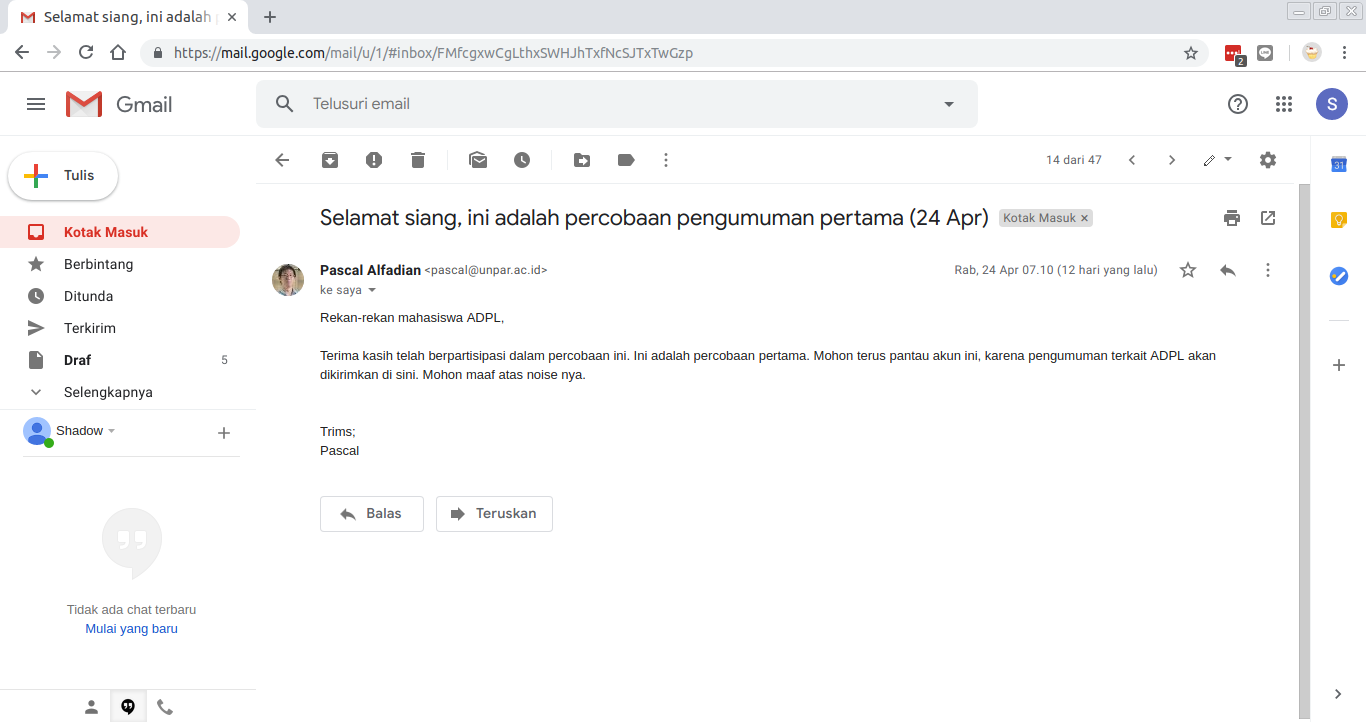
\includegraphics[width=\textwidth]{email-24-april.png}  
	\caption[Email pada tanggal 24 April 2019 oleh Bapak Pascal]]{Email pada tanggal 24 April 2019 oleh Bapak Pascal} 
	\label{fig:email-24Apr} 
\end{figure}                         

\subsubsection{Hasil Pengujian}
Setelah masa pengujian berakhir, responden yang mengisi kuesioner adalah 72 responden yang terdiri dari 70 mahasiswa dan 2 dosen. Dari 70 mahasiswa tersebut, 42 mahasiswa mengaku mendapatkan notifikasi LINE dan 28 mahasiswa mengaku tidak mendapatkan notifikasi LINE. Namun, karena memakai plan developer, maksimal pengikut akun bot tersebut adalah 50 orang. Sehingga perkiraan mahasiswa yang tidak mendapatkan notifikasi LINE setelah mengikuti bot LINE adalah 8 mahasiswa.

Dari 42 mahasiswa yang mengaku mendapatkan notifikasi LINE, 30 mahasiswa mengaku dapat membuka url yang tercantum di notifikasi pengumuman dan 12 mahasiswa mengaku tidak dapat membuka url yang tercantum di notifikasi pengumuman. Dari kolom saran beberapa mahasiswa melaporkan bahwa mereka tidak dapat login ke shadowtape. Berikut jawaban mereka di kolom saran :
\begin{itemize}
  \item Jawaban untuk kolom saran dari 2017730022@student.unpar.ac.id : "terdapat beberapa error dalam login, dimana email saya (@student.unpar) tidak memiliki akses"
  \item Jawaban untuk kolom saran dari 2017730047@student.unpar.ac.id : "memperbaiki url login yang dikirimkan di shadowtape"
  \item Jawaban untuk kolom saran dari 2017730011@student.unpar.ac.id : "saran saya, usahakan tidak menggunakan aplikasi luar lain seperti LINE. dikarenakan tidak semua orang menggunakan line"
  \item Jawaban untuk kolom saran dari 2017730037@student.unpar.ac.id : "Link yang dibuka langsung dari line tidak memiliki hak akses"
  \item Jawaban untuk kolom saran dari 2017730044@student.unpar.ac.id : "Log in masih tidak dapat dilakukan, terdapat pernyataan bahwa "alamat email" tidak memiliki hak akses ke pengumuman. Contohnya email yang saya gunakan "2017730044@student.unpar.ac.id tidak memiliki hak akses ke pengumuman"
\end{itemize}

Setelah memeriksa respon mereka di kuesioner untuk pertanyaan "Apakah Anda dapat membuka url yang dicantumkan di notifikasi pengumuman?", mahasiswa dengan alamat email 2017730022@student.unpar.ac.id dan 2017730011@student.unpar.ac.id menjawab "Tidak" untuk pertanyaan tersebut. Sementara mahasiswa dengan alamat email 2017730047@student.unpar.ac.id, 2017730037@student.unpar.ac.id, dan 2017730044@student.unpar.ac.id menjawab "Ya". Kemungkinan beberapa mahasiswa menjawab "Tidak" karena tidak dapat login ke shadowtape dengan alasan hak akses. Penyebab tidak bisa login tersebut diperkirakan karena shadowtape belum mengenali pola alamat email student yang baru sebagai alamat email yang berhak login di shadowtape. 

Masalah tersebut sudah ditangani di repository induk, namun penulis belum menyalin kode untuk menangani masalah tersebut ke repository penulis pada saat pengujian dimulai (24 April 2019). Pada tanggal 25 April 2019 penulis mendapatkan laporan adanya masalah tersebut melalui jalur pribadi. Segera setelah menerima laporan tersebut, penulis melakukan "git pull" ke repository induk. Setelahnya, penulis mengirimkan email ke shadowbluetape@gmail.com yang berisi pengumuman bahwa masalah tersebut telah diperbaiki. Namun, berdasarkan laporan dari kuesioner, beberapa mahasiswa masih menemukan masalah ini.

Dari 30 mahasiswa yang dapat membuka url yang dicantumkan di notifikasi pengumuman, 21 mahasiswa mengaku diarahkan kembali ke url tersebut setelah login dan 9 mahasiswa mengaku diarahkan ke halaman lain setelah login. Penulis memperkirakan alasan 9 mahasiswa tersebut diarahkan ke halaman lain karena masalah hak akses juga.

Dari 2 dosen yang menjawab kuesioner ini, 1 dosen menjawab dapat melihat pengumuman yang ia kirimkan di shadowtape dan 1 dosen menjawab tidak dapat melihat pengumuman yang ia kirimkan di shadowtape. Dosen yang menjawab tidak dapat melihat pengumuman yang ia kirimkan adalah dosen yang tidak pernah mengirimkan email ke shadowbluetape@gmail.com. Dosen yang menjawab dapat melihat pengumuman yang ia kirimkan di shadowtape menjawab bahwa judul dan isi pengumuman sesuai dengan subjek dan isi email yang ia kirimkan.

Untuk hasil uji usabilitas menggunakan System Usability Scale, penulis merangkum hasilnya di Gambar~\ref{fig:summary-Diagram-Skor-SUS}. Rata-rata skor System Usability Scale menurut hasil kuesioner adalah 60,34. Angka tersebut menunjukkan bahwa usabilitas fitur Kolektor Pengumuman Informatika cukup bagus, namun perlu ditingkatkan.

\begin{figure}[H]
	\centering  
	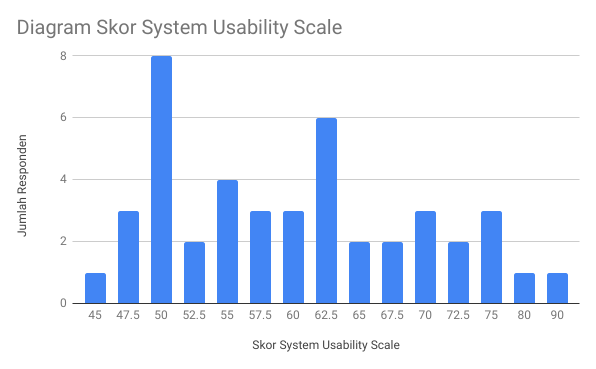
\includegraphics[scale=0.5]{./Survey-Summary/Diagram-Skor-SUS.png}
	\caption[Diagram Skor System Usability Scale]{Diagram Skor System Usability Scale} 
	\label{fig:summary-Diagram-Skor-SUS} 
\end{figure}

Selain masalah hak akses saat login, penulis mendapatkan masukan-masukan lain dari kolom saran :
\begin{itemize}
  \item Masukan dari keenan.leman@unpar.ac.id : "Tidak bisa /"add friend" karena akun telah mencapai batas banyak teman."
  
  Tanggapan dari penulis : Hal ini wajar terjadi karena plan untuk LINE@ yang dipakai di skripsi ini adalah plan developer. Plan ini membatasi pengikut akun bot sampai 50 teman. Masalah ini bisa diatasi dengan pembaruan kebijakan baru oleh LINE. Kebijakan baru tersebut menyatakan bahwa LINE@ akan ditiadakan dan dimigrasikan ke layanan baru LINE : LINE Official Account. Kedua layanan tersebut serupa, namun pengenaan biayanya berbeda. LINE@ memakai jumlah teman untuk pengenaan biayanya sedangkan LINE Official Account memakai jumlah pesan yang dikirimkan untuk pengenaan biayanya.

  Sekilas LINE Official Account dapat menangani masalah ini,namun LINE Official Account dirilis tidak lama sebelum pengujian ini dilakukan (10 April 2019). Penulis tidak memiliki waktu yang cukup untuk mempelajari lebih lanjut layanan baru ini. Walaupun migrasi dari LINE@ ke LINE Official Account akan tetap terjadi, migrasi ini baru akan dilakukan pada bulan Juni 2019.

  \item Masukan dari segi tampilan oleh 7316027@student.unpar.ac.id : "Lebih diperbagus tampilannya sehingga menarik user untuk menggunakannya" dan 7316025@student.unpar.ac.id : "Lebih user friendly"
  
  Tanggapan dari penulis : Karena skripsi ini lebih mengedepankan fungsionalitas, penulis tidak terlalu memperhatikan tampilan fitur. Namun, masukan ini dapat ditambahkan sebagai saran apabila ada yang ingin melanjutkan penelitian ini.
  
  \item Masukan dari 2017730008@student.unpar.ac.id : "Fitur ini bagus, memudahkan mahasiswa dalam menerima notifikasi email. Namun, waktunya sebaiknya tidak hanya pada jam 12 siang karena waktu tersebut adalah saat orang-orang makan siang yang mungkin saja sedang tidak membuka gadget/aplikasi Line pada khususnya."
  
  Tanggapan dari penulis : Setelah berdiskusi dengan pembimbing yang telah meminjamkan kartu kreditnya untuk menambahkan add on Heroku Scheduler, penulis dan pembimbing memutuskan untuk mengganti jadwal Cron dari tiap hari jam 12 menjadi tiap jam. Keputusan tersebut diambil setelah melihat pemakaian dyno yang tidak terlalu besar.
\end{itemize}